\documentclass[aspectratio=169]{beamer}
\usepackage{xcolor}
\usepackage{luatexja}
\usepackage[haranoaji]{luatexja-preset}
\usepackage{fontspec}
\usepackage{setspace}
\usepackage{amsmath, amssymb, amsthm}
\usepackage{tabularx}
\usepackage{booktabs}
\usepackage{makecell}
\setstretch{1.2}

\definecolor{MyBlue}{HTML}{d8fa00}
\definecolor{MyGray}{HTML}{f28112}
\IfFontExistsTF{Noto Sans JP}{\setsansjfont{Noto Sans JP}}{}

\setbeamercolor{title}{fg=white,bg=MyBlue}
\setbeamercolor{frametitle}{fg=white,bg=MyGray}
\setbeamercolor{block title}{bg=MyBlue}
\setbeamercolor{block body}{bg=MyBlue!8}
\setbeamertemplate{navigation symbols}{}
\setbeamertemplate{footline}[frame number]

% ---------- Macros ----------
\newcommand{\floor}[1]{\mathrm{Floor}\!\left(#1\right)}
\newcommand{\ceil}[1]{\mathrm{Ceil}\!\left(#1\right)}
\newcommand{\param}[1]{#1_{\mathrm{snap}}}
\newcolumntype{C}{>{\centering\arraybackslash}X}

\begin{document}

%%%%%%%%%%%%%%%%%%%%%%%%%%%%%%%%%%%%%%%%%%%%%%%%%%%%%%%%%%%%%%%%%%%%%%%%
\begin{frame}{はじめに}
異常ダメージは異常蓄積値とそのときの攻撃力, ダメージボーナス, 異常マスタリー等の加重平均から求められる.
異常蓄積値はエージェントのスキルごとに設定されているが, ゲーム内のステータス画面で確認できない.

そこで本稿では異常蓄積値を考慮した狂咲ダメージの計算式からスキルごとの異常蓄積値と敵の異常蓄積値上限の近似値を算出する方法の１つを紹介する.
\end{frame}

\begin{frame}{はじめに}
\begin{block}{今回の内容}
\begin{enumerate}
	\item 狂咲ダメージ計算方法(異常蓄積考慮無し)
	\item 狂咲ダメージ計算方法(異常蓄積考慮有り)
	\item スキルの異常蓄積値近似方法
	\item 敵の異常蓄積値上限の近似方法
\end{enumerate}
\end{block}
※あくまで妄想エンジェルと危局の血狩りの掃除屋を対象とした具体例の紹介が目的
\end{frame}
%%%%%%%%%%%%%%%%%%%%%%%%%%%%%%%%%%%%%%%%%%%%%%%%%%%%%%%%%%%%%%%%%%%%%%%%
\begin{frame}{狂咲ダメージ計算方法(異常蓄積考慮無し)}
\vspace{-0.5em}
\begin{block}{狂咲ダメージの因子}
\begin{tabularx}{\linewidth}{clX}
1 & 攻撃力 & エージェント基礎攻撃力, 攻撃バフ \\
2 & ダメージボーナス & 初期値 $100$ とディスク5番メイン等の総和 \\
3 & 異常マスタリー & エージェントごとの初期値とサブステ等の総和 \\
4 & 防御補正 & 敵防御力・防御ダウン・貫通値・貫通率等 \\
5 & 属性耐性 & 敵の弱点属性による補正等 \\
6 & ブレイク倍率 & ブレイク時の補正 \\
7 & 異常ダメージボーナス & 異常ダメージ専用のボーナス補正 \\
8 & レベル補正 & エージェントレベル60では$2$ \\
9 & 異常ダメージ倍率 & 属性毎に設定された固定値 \\
10 & 狂咲倍率 & エージェント毎の倍率 \\
11 & 狂咲ダメージボーナス & 狂咲ダメージ専用のボーナス補正 \\
12 & 別枠乗算 & 上記以外の項目 \\
\end{tabularx}
\end{block}
\end{frame}



%%%%%%%%%%%%%%%%%%%%%%%%%%%%%%%%%%%%%%%%%%%%%%%%%%%%%%%%%%%%%%%%%%%%%%%%
\begin{frame}{狂咲ダメージ計算方法(異常蓄積考慮無し)}

\begin{block}{アリア（妄想エンジェル編成）の攻撃力計算例}
\small
\begin{tabularx}{\linewidth}{@{}l l X@{}}
区分 & 値 & 内訳 \\
\midrule
初期値 & $1576$ & 基礎攻撃力： $788$, コアスキル$75$, アリア餅： $713$\\
\midrule
戦闘前 乗算バフ & $1.63$ & \makecell[l]{サブステータス： $63$}\\
\midrule
戦闘時 乗算バフ & $1.1$ & 千夏餅：$10$ \\
\midrule
戦闘前 加算バフ & $335$ & ディスク2番メイン： $316$, サブステータス実数値： $19$ \\
\midrule
戦闘時 加算バフ & $1100$ & 千夏コアパッシブ： $1050$, エーテルベール: $50$ \\
\midrule
\end{tabularx}
\vspace{0em}
\[
  \text{攻撃力}  = \floor{1576\times 1.63 + 335}\times 1.1 + 1100 = 4293.3
\]
\end{block}
ここで正の実数 $x$ に対し,  $ \floor{x} $ は $x$ の整数部分を表す.
\end{frame}

%%%%%%%%%%%%%%%%%%%%%%%%%%%%%%%%%%%%%%%%%%%%%%%%%%%%%%%%%%%%%%%%%%%%%%%%

\begin{frame}{狂咲ダメージ計算方法(異常蓄積考慮無し)}
\begin{block}{アリア（妄想エンジェル編成）のダメージボーナス計算例}
\small
\begin{tabularx}{\linewidth}{@{}l l X@{}}
区分 & 値 & 内訳 \\
\midrule
初期値 & $100$ & 共通値$100$ \\
\midrule
戦闘前バフ & $30$ & ディスク5番メイン: $30$ \\
\midrule
戦闘時バフ & $143$ & \makecell[l]{千夏餅: $25$, 南宮コアパ: $25$, 南宮餅: $30$, アリア餅: $20$ \\ パエ4: $25$, 月光4: $18$ }\\
\midrule
\end{tabularx}

\vspace{0.4em}
\[
  \text{ダメージボーナス} = 100 + 30 + 143 = 273
\]
\end{block}
\end{frame}

%%%%%%%%%%%%%%%%%%%%%%%%%%%%%%%%%%%%%%%%%%%%%%%%%%%%%%%%%%%%%%%%%%%%%%%%

\begin{frame}{狂咲ダメージ計算方法(異常蓄積考慮無し)}
\begin{block}{アリア（妄想エンジェル編成）の異常マスタリー計算例}
\small
\begin{tabularx}{\linewidth}{@{}l l X@{}}
区分 & 値 & 内訳 \\
\midrule
初期値 & $116$ & アリア初期値: $116$ \\
\midrule
戦闘前バフ & $248$ & ディスク4番メイン: $92$, サブステ: $126$, ケイオス2: $30$ \\
\midrule
戦闘時バフ & $225$ & \makecell[l]{アリア餅: $90$, アリアコアパ: $90$, パエ4: $45$}\\
\midrule
\end{tabularx}

\vspace{0.4em}
\[
  \text{異常マスタリー} = 116 + 248 + 225 = 589
\]
\end{block}
\end{frame}

%%%%%%%%%%%%%%%%%%%%%%%%%%%%%%%%%%%%%%%%%%%%%%%%%%%%%%%%%%%%%%%%%%%%%%%%
\begin{frame}{狂咲ダメージ計算方法(異常蓄積考慮無し)}
\begin{block}{防御補正の計算式}
\small
\begin{itemize}
  \item $D_{\mathrm{enemy}}$：敵防御力. 敵の種類とレベルで定まる.
  \item $r_{\mathrm{pen}}$：貫通率
  \item $v_{\mathrm{pen}}$：貫通値
  \item $r_{\mathrm{down}}$：防御ダウン, 防御無視
  \item $L$：エージェントレベル補正値. エージェントレベル 60 のときは $L=794$ 
\end{itemize}
\[
\begin{aligned}
\text{デバフ後敵防御力} E
&=
D_{\mathrm{enemy}}
(1-r_{\mathrm{pen}})
(1-r_{\mathrm{down}})
-
v_{\mathrm{pen}}
\\
\text{防御補正}
&=
\frac{L}{E+L}
\end{aligned}
\]
\end{block}


\end{frame}

%%%%%%%%%%%%%%%%%%%%%%%%%%%%%%%%%%%%%%%%%%%%%%%%%%%%%%%%%%%%%%%%%%%%%%%%

\begin{frame}{狂咲ダメージ計算方法(異常蓄積考慮無し)}
\begin{block}{アリア（妄想エンジェル編成）の防御補正計算例}
\small
\begin{tabularx}{\linewidth}{@{}l l X@{}}
区分 & 値 & 内訳 \\
\midrule
敵防御力 & $84.6$ & 訓練所タナトスレベル10: $84.6$ \\
\midrule
貫通率 & $0$ &  \\
\midrule
貫通値 & $18$ & サブステ: $18$\\
\midrule
防御ダウン & $0$ & \\
\midrule
エージェントレベル補正値 & $794$ & \\
\midrule
\end{tabularx}

\vspace{0.4em}
\[
\begin{aligned}
\text{デバフ後敵防御力} 
&=
84.6\times
(1-0)
(1-0)
-
18 = 66.6
\\
\text{防御補正}
&=
\frac{794}{66.6+794} = \frac{794}{860.6} 
\end{aligned}
\]
\end{block}
\end{frame}

%%%%%%%%%%%%%%%%%%%%%%%%%%%%%%%%%%%%%%%%%%%%%%%%%%%%%%%%%%%%%%%%%%%%%%%%

\begin{frame}{狂咲ダメージ計算方法(異常蓄積考慮無し)}
\begin{block}{アリア（妄想エンジェル編成）の属性耐性計算例}
\small
\begin{tabularx}{\linewidth}{@{}l l X@{}}
区分 & 値 & 内訳 \\
\midrule
初期値 & $100$ & 共通初期値: $100$ \\
\midrule
敵固有加算値 & $20$ & タナトス(エーテル弱点): $20$ \\
\midrule
デバフ & $0$ & \\
\midrule
\end{tabularx}

\vspace{0.4em}
\[
  \text{属性耐性} = 100 + 20 + 0 = 120
\]
\end{block}
\end{frame}

%%%%%%%%%%%%%%%%%%%%%%%%%%%%%%%%%%%%%%%%%%%%%%%%%%%%%%%%%%%%%%%%%%%%%%%%

\begin{frame}{狂咲ダメージ計算方法(異常蓄積考慮無し)}
\begin{block}{アリア（妄想エンジェル編成）のブレイク倍率計算例}
\small
\begin{tabularx}{\linewidth}{@{}l l X@{}}
区分 & 値 & 内訳 \\
\midrule
初期値 & $200$ & 訓練所タナトス初期値: $200$ \\
\midrule
デバフ & $60$ &千夏コアパッシブ: $30$, 南宮追加能力: $30$ \\
\midrule
\end{tabularx}

\vspace{0.4em}
\[
  \text{ブレイク倍率} =200 + 60 = 260
\]
\end{block}
\end{frame}

%%%%%%%%%%%%%%%%%%%%%%%%%%%%%%%%%%%%%%%%%%%%%%%%%%%%%%%%%%%%%%%%%%%%%%%%

\begin{frame}{狂咲ダメージ計算方法(異常蓄積考慮無し)}
ここでいう異常ダメージボーナスとは, アリア餅の「状態異常ダメージ$+10\%$」と同じ項目として加算されるものを指す.
\begin{block}{アリア（妄想エンジェル編成）の異常ダメージボーナス計算例}
\small
\begin{tabularx}{\linewidth}{@{}l l X@{}}
区分 & 値 & 内訳 \\
\midrule
初期値 & $100$ & 共通初期値: $100$ \\
\midrule
バフ・デバフ & $10$ & アリア餅: $10$ \\
\midrule
\end{tabularx}

\vspace{0.4em}
\[
  \text{異常ダメージボーナス} = 100 + 10 = 110
\]
\end{block}
※他には柚葉追加能力が同じ項目としてある.
\end{frame}

%%%%%%%%%%%%%%%%%%%%%%%%%%%%%%%%%%%%%%%%%%%%%%%%%%%%%%%%%%%%%%%%%%%%%%%%

\begin{frame}{狂咲ダメージ計算方法(異常蓄積考慮無し)}
今回, レベル補正と異常ダメージ倍率は固定値とみなすため詳細は省略する.
\begin{block}{アリア（妄想エンジェル編成）のレベル補正と異常ダメージ倍率例}
\small
\begin{tabularx}{\linewidth}{@{}l l X@{}}
区分 & 値 & 備考 \\
\midrule
レベル補正 & $200$ & アリアレベル$60$ \\
\midrule
異常ダメージ倍率 & $62.5$ & 侵蝕ダメージ倍率固定値 \\
\end{tabularx}
\end{block}
\end{frame}


%%%%%%%%%%%%%%%%%%%%%%%%%%%%%%%%%%%%%%%%%%%%%%%%%%%%%%%%%%%%%%%%%%%%%%%%

\begin{frame}{狂咲ダメージ計算方法(異常蓄積考慮無し)}
狂咲ダメージ倍率の算出方法はキャラクターの技ごとによって異なる. アリアの狂咲ダメージ倍率はコアスキルレベルによる基礎倍率と異常掌握値から求まる.
\begin{block}{アリア（妄想エンジェル編成）の狂咲ダメージ倍率例}
\small
\begin{tabularx}{\linewidth}{@{}l l X@{}}
区分 & 値 & 備考 \\
\midrule
基礎倍率 & $27.5$ & コアスキルF, 侵蝕状態異常時 \\
\midrule
異常掌握値 & $253$ & コアスキルF, パエ2, ディスク6番メイン \\
\midrule
\end{tabularx}
\vspace{0.4em}
\[
  \text{狂咲ダメージ倍率} = \frac{27.5 \times 253}{10} = 695.75
\]
\end{block}
\end{frame}

%%%%%%%%%%%%%%%%%%%%%%%%%%%%%%%%%%%%%%%%%%%%%%%%%%%%%%%%%%%%%%%%%%%%%%%%

\begin{frame}{狂咲ダメージ計算方法(異常蓄積考慮無し)}
ここでいう狂咲ダメージボーナスとは,
アリアのコアパッシブによるブレイク時バフ \(50\%\) や,
危局バフ「続変」の \(30\%\) など,
同一項目として加算される補正を指す.
\begin{block}{アリア（妄想エンジェル編成）の狂咲ダメージボーナス例}
\small
\begin{tabularx}{\linewidth}{@{}l l X@{}}
区分 & 値 & 内訳 \\
\midrule
初期値 & $100$ &  \\
\midrule
バフ・デバフ & $50$ & アリアコアパッシブ \\
\end{tabularx}
\vspace{0.4em}
\[
  \text{狂咲ダメージボーナス} = 100 + 50 = 150
\]
\end{block}
\end{frame}

%%%%%%%%%%%%%%%%%%%%%%%%%%%%%%%%%%%%%%%%%%%%%%%%%%%%%%%%%%%%%%%%%%%%%%%%

\begin{frame}{狂咲ダメージ計算方法(異常蓄積考慮無し)}
これまでに挙げた項目のいずれにも属さないものを別枠乗算値としてまとめる.
今回対象となるのは危局強襲戦における血狩りの掃除屋エネミー詳細にある「受ける状態異常ダメージ$+15\%$」のことを指す.

\end{frame}

%%%%%%%%%%%%%%%%%%%%%%%%%%%%%%%%%%%%%%%%%%%%%%%%%%%%%%%%%%%%%%%%%%%%%%%%

\begin{frame}{狂咲ダメージ計算方法(異常蓄積考慮無し)}
これまで算出したすべての項目の積は以下のようになる.
攻撃力と防御補正以外はすべて百分率表記から割合としての数値に戻すため $100$ で割っている.
\[
\begin{aligned}
&4293.3
\times
\frac{273}{100}
\times
\frac{589}{100}
\times
\frac{794}{860.6}
\times
\frac{120}{100}
\times
\frac{260}{100}
\times
\frac{110}{100}
\times
\frac{200}{100}
\times
\frac{62.5}{100}
\times
\frac{695.75}{100}
\times
\frac{150}{100}
\\
&=
2851609.844...
\end{aligned}
\]
\end{frame}

%%%%%%%%%%%%%%%%%%%%%%%%%%%%%%%%%%%%%%%%%%%%%%%%%%%%%%%%%%%%%%%%%%%%%%%%
\begin{frame}{狂咲ダメージ計算方法(異常蓄積考慮無し)}
このようにパラメータの積を計算して得られる値を \textbf{計算ダメージ} と呼ぶことにする.
この一方で, 実際にゲーム上に表示されるダメージを \textbf{表示ダメージ} と呼ぶことにする.  
本稿では, 計算ダメージを整数に切り上げた値が表示ダメージになると仮定する.
\begin{block}{仮定：計算ダメージと表示ダメージの関係}
計算ダメージ $d$ と表示ダメージ $D$ は以下を満たす.
\[
  D = \ceil{d}
\]
\end{block}
\[
  \text{例:} 2851610 = \ceil{2851609.844...}
\]
\end{frame}

%%%%%%%%%%%%%%%%%%%%%%%%%%%%%%%%%%%%%%%%%%%%%%%%%%%%%%%%%%%%%%%%%%%%%%%%
\begin{frame}{狂咲ダメージ計算方法(異常蓄積考慮有り)}
エージェントの技ごとに異常蓄積基礎値が設定されている. 
これはエージェントレベルやスキルレベルに依存しない.
\begin{block}{異常蓄積値の計算式}
\small
\begin{itemize}
  \item $q$：技ごとに設定された基礎異常蓄積値
  \item $P_{\mathrm{anom}}$：異常掌握値
  \item $B_{\mathrm{acc}}$：異常蓄積効率
  \item $R_{\mathrm{enemy}}$：敵側の属性耐性
\end{itemize}
\[
\begin{aligned}
t
&=
q
\times
\frac{P_{\mathrm{anom}}}{100}
\times
\frac{B_{\mathrm{acc}}}{100}
\times
\frac{R_{\mathrm{enemy}}}{100}
\end{aligned}
\]
\end{block}
\end{frame}

%%%%%%%%%%%%%%%%%%%%%%%%%%%%%%%%%%%%%%%%%%%%%%%%%%%%%%%%%%%%%%%%%%%%%%%%

\begin{frame}{狂咲ダメージ計算方法(異常蓄積考慮有り)}
異常発生までに複数回攻撃した場合, 攻撃力は単純平均ではなく,
各攻撃が与えた異常蓄積値による加重平均で計算する.

\begin{block}{攻撃力の加重平均}
\small
第 $i$ 回目の攻撃$(i = 1, ..., n)$の攻撃力を $X_i$, 異常蓄積値を $t_i$ とする.
このとき, 異常ダメージ計算に使う攻撃力 $\bar{X}$ は次のようになる.

\[
\begin{aligned}
T
&=
t_1+t_2+\cdots+t_n
\\
\bar{X}
&=
\frac{
t_1X_1+t_2X_2+\cdots+t_nX_n
}{
t_1+t_2+\cdots+t_n
}
\end{aligned}
\]

\end{block}

ここで $T$ は敵の異常蓄積値上限である. 

\end{frame}
%%%%%%%%%%%%%%%%%%%%%%%%%%%%%%%%%%%%%%%%%%%%%%%%%%%%%%%%%%%%%%%%%%%%%%%%
\begin{frame}{狂咲ダメージ計算方法(異常蓄積考慮有り)}
一部の項目は異常蓄積時点の値を加重平均し,
一部の項目はダメージ発生時点の値を使う.

\begin{columns}[T,onlytextwidth]
\begin{column}{0.49\linewidth}
\begin{block}{スナップショットする項目}
\small
\begin{itemize}
  \item 攻撃力
  \item ダメージボーナス
  \item 異常マスタリー
  \item 貫通値
  \item 貫通率
\end{itemize}
\end{block}
\end{column}

\begin{column}{0.49\linewidth}
\begin{block}{リアルタイムで計算される項目}
\small
\begin{itemize}
  \item ブレイク倍率
  \item 異常ダメージボーナス
  \item 狂咲倍率
  \item 狂咲ダメージボーナス
\end{itemize}
\end{block}
\end{column}
\end{columns}

\vspace{0.5em}
\small
※上記以外の項目についてはスナップショットされるかどうかは今回の調査対象外.

\end{frame}
%%%%%%%%%%%%%%%%%%%%%%%%%%%%%%%%%%%%%%%%%%%%%%%%%%%%%%%%%%%%%%%%%%%%%%%%

\begin{frame}{スキルの異常蓄積値近似方法}
求めたいスキルの異常蓄積値(異常掌握などの乗算項目すべて込み)を $t$ とし, 敵の異常蓄積値上限を $T$ とする.
最初に攻撃力 $X$ の状態でスキルを当てた後, 攻撃力を $\Delta x$ だけバフした後に残りの異常蓄積値をためた場合, 攻撃力の加重平均は

\[
\bar{X}
=
\frac{
  tX + (T-t)(X+\Delta x)
}{
  T
}
=
X + \left(1-\frac{t}{T}\right)\Delta x
\]

となる.
攻撃力以外のバフはないとし, 他の因子の積を定数 $C$ とおくと, 計算ダメージ $d$は
\[
\begin{aligned}
d
=
C\bar{X}
=
C\left\{
X + \left(1-\frac{t}{T}\right)\Delta x
\right\}
\end{aligned}
\]

となる.
\end{frame}
%%%%%%%%%%%%%%%%%%%%%%%%%%%%%%%%%%%%%%%%%%%%%%%%%%%%%%%%%%%%%%%%%%%%%%%%
\begin{frame}{スキルの異常蓄積値近似方法}
計算ダメージと表示ダメージの仮定 $D = \ceil{d}$ から $D-1 < d \le D $ となるので, この範囲で $\frac{t}{T}$ について解くと以下のようになる.

\begin{block}{相対値$\frac{t}{T}$ の範囲}
\small
\[
\frac{
C(X+\Delta x)-D
}{
C\Delta x
}
\le
\frac{t}{T}
<
\frac{
C(X+\Delta x)-(D-1)
}{
C\Delta x
}
\]
\end{block}

\small
このようにして相対値の範囲を求めることができるが, 絶対値 $t$ を求めるには敵の異常蓄積値上限 $T$ の値が必要である.

\end{frame}
%%%%%%%%%%%%%%%%%%%%%%%%%%%%%%%%%%%%%%%%%%%%%%%%%%%%%%%%%%%%%%%%%%%%%%%%
\begin{frame}{スキルの異常蓄積値近似方法}
通常エネミーなどの異常蓄積値上限は以下のようにして求められているのでこの数値を使用する.
なお, 危局ボスの異常蓄積値上限は画像の値より大きくずれることが多い.
\begin{figure}
  \centering
  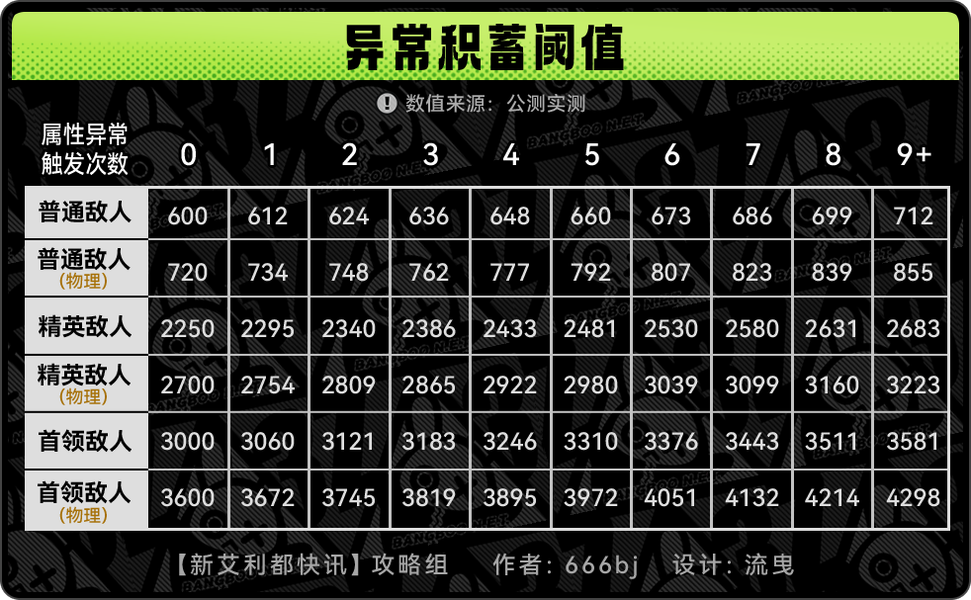
\includegraphics[width=0.6\linewidth]{enemy.png}
\end{figure}
\end{frame}
%%%%%%%%%%%%%%%%%%%%%%%%%%%%%%%%%%%%%%%%%%%%%%%%%%%%%%%%%%%%%%%%%%%%%%%%
\begin{frame}{スキルの異常蓄積値近似方法}

\begin{block}{絶対値の範囲}
\small
前のスライドで求めた範囲に対して, 不等式全体を $T$ 倍すると,
スキルの異常蓄積値 $t$ の範囲が求まる.
\[
\frac{
C(X+\Delta x)-D
}{
C\Delta x
}
\cdot T
\le
t
<
\frac{
C(X+\Delta x)-(D-1)
}{
C\Delta x
}
\cdot T
\]

また, 区間の幅は以下のようになる.

\[
\begin{aligned}
\Delta t
=
T\cdot
\frac{
C(X+\Delta x)-(D-1)
}{
C\Delta x
}
-
T\cdot
\frac{
C(X+\Delta x)-D
}{
C\Delta x
}
=
\frac{T}{C\Delta x}
\end{aligned}
\]
\end{block}

\small
つまり攻撃力以外の積 $C$ と攻撃力のバフ量 $\Delta x$ が大きいほど区間幅は狭くなり, より高精度で近似することができる.

\end{frame}
%%%%%%%%%%%%%%%%%%%%%%%%%%%%%%%%%%%%%%%%%%%%%%%%%%%%%%%%%%%%%%%%%%%%%%%%
\begin{frame}{スキルの異常蓄積値近似方法}
敵は訓練所タナトスとする.
また, 攻撃力バフ $\Delta x$ の値を大きくするため, アリア・千夏・シーザー編成で調査する.
\begin{block}{アリア（千夏・シーザー編成）の攻撃力バフ例}
\small
\begin{tabularx}{\linewidth}{@{}l l X@{}}
区分 & 値 & 内訳・備考 \\
\midrule
敵異常蓄積値上限 & $2250$ & 訓練所タナトス \\
\midrule
攻撃力バフ & $2100$ & 千夏コアパ: $1050$, シーザー追加能力: $1000$, エーテルベール: $50$ \\
\midrule
\end{tabularx}
\vspace{0.4em}
\[
\begin{aligned}
  \text{敵異常蓄積値上限} T &= 2250\\
  \text{攻撃力バフ} \Delta x&= 2100
\end{aligned}
\]
\end{block}
※ここでは攻撃力だけバフをさせる必要があるため, ダメージボーナスもバフしてしまう柚葉や千夏餅, 月光4を使用することができない.
\end{frame}
%%%%%%%%%%%%%%%%%%%%%%%%%%%%%%%%%%%%%%%%%%%%%%%%%%%%%%%%%%%%%%%%%%%%%%%%
\begin{frame}{スキルの異常蓄積値近似方法}
ダメージボーナスや異常マスタリーを固定させるため, 先ほどの例からディスクと音動機を調整する.
その結果変更があった項目と値は以下のとおりである.
\begin{block}{アリア（千夏・シーザー編成）の因子例}
\small
\begin{tabularx}{\linewidth}{@{}l l X@{}}
区分 & 値 & 内訳 \\
\midrule
戦闘前攻撃力 & $2951$ &南宮餅, サブステ等  \\
\midrule
ダメージボーナス & $140$ &ディスク5番メイン, アリア2セット  \\
\midrule
異常マスタリ & $427$ & ケイオス2セット, サブステ: $99$ 等 \\
\midrule
ブレイク倍率 & $230$ & 千夏コアパ  
\end{tabularx}
\end{block}
\end{frame}

%%%%%%%%%%%%%%%%%%%%%%%%%%%%%%%%%%%%%%%%%%%%%%%%%%%%%%%%%%%%%%%%%%%%%%%%
\begin{frame}{スキルの異常蓄積値近似方法}
アリアの「強化特殊スキル：もーそーに落ちて」の基礎値を求める.
表示ダメージ $D$ は $745881$ となるので $t$ の範囲は以下のようになる:
\[
\begin{aligned}
&
\frac{
C(X+\Delta x)-D
}{
C\Delta x
}
\cdot T 
= 1387.4507,
\\[1.0em]
&
\frac{
C(X+\Delta x)-(D-1)
}{
C\Delta x
}
\cdot T 
= 1387.456096.
\end{aligned}
\]

\[
1387.4507
\le
t
<
1387.456096
\]
さらに異常掌握値 $2.53$ と属性耐性 $1.2$ で割れば, スキルの基礎値 $q$ は以下の範囲になる.
\[
456.999572
\le
q
<
457.0013491
\]
\end{frame}



%%%%%%%%%%%%%%%%%%%%%%%%%%%%%%%%%%%%%%%%%%%%%%%%%%%%%%%%%%%%%%%%%%%%%%%%
\begin{frame}{スキルの異常蓄積値近似方法}
後は好みの問題で, ここではアリアの「強化特殊スキル：もーそーに落ちて」基礎値を  $457.00$ とする.
他も同様の方法で小数第二位までを求めた結果の一部を以下に記す.
\begin{block}{アリアのスキル基礎蓄積値}
\small
\begin{tabularx}{\linewidth}{@{}l l X@{}}
スキル名 & 基礎値 \\
\midrule
【通常攻撃】スイートリズム・1段 & $22.80$ \\
【通常攻撃】スイートリズム・2段 & $46.57$ \\
【通常攻撃】スイートリズム・3段 & $58.04$ \\
【通常攻撃】スイートリズム・4段 & $134.00$ \\
【ダッシュ攻撃】レガートステップ & $20.81$ \\
【通常攻撃】絶対音感・3段チャージ攻撃 & $130.00$ \\
【通常攻撃】絶対音感・3段チャージ攻撃（協力攻撃） & $149.50$ \\
【強化特殊スキル】秒でハマって & $486.20$ \\
【連携スキル】夢のコラボ & $542.46$
\end{tabularx}
\end{block}
\end{frame}

%%%%%%%%%%%%%%%%%%%%%%%%%%%%%%%%%%%%%%%%%%%%%%%%%%%%%%%%%%%%%%%%%%%%%%%%
\begin{frame}{スキルの異常蓄積値近似方法}
似た方法で求めた南宮の基礎値の一部も以下に記す.

\begin{block}{南宮のスキル基礎蓄積値}
\small
\begin{tabularx}{\linewidth}{@{}l l X@{}}
スキル名 & 基礎値 \\
\midrule
【通常攻撃】流星ステップ・1段 & $59.33$ \\
【通常攻撃】流星ステップ・2段 & $62.15$ \\
【通常攻撃】流星ステップ・3段 & $129.07$ \\
【通常攻撃】プリティーマインアタック・1段チャージ攻撃 & $40.00$ \\
【通常攻撃】プリティーマインアタック・2段チャージ攻撃 & $191.63$ \\
【通常攻撃】プリティーマインアタック・3段チャージ攻撃（協力攻撃） & $373.36$ \\
【強化特殊スキル】とびっきり重いラブ & $463.27$ 
\end{tabularx}
\end{block}
\end{frame}

%%%%%%%%%%%%%%%%%%%%%%%%%%%%%%%%%%%%%%%%%%%%%%%%%%%%%%%%%%%%%%%%%%%%%%%%
\begin{frame}{敵の異常蓄積値上限の近似方法}
求めたスキル異常蓄積値を用いて危局ボス「血狩りの掃除屋」の異常蓄積値上限を求める.
先ほど得た式
\[
\frac{
C(X+\Delta x)-D
}{
C\Delta x
}
\le
\frac{t}{T}
<
\frac{
C(X+\Delta x)-(D-1)
}{
C\Delta x
}
\]
を $T$ について解くと,

\[
\frac{
t C\Delta x
}{
C(X+\Delta x)-(D-1)
}
<
T
\le
\frac{
t C\Delta x
}{
C(X+\Delta x)-D
}
\]
となる.
\end{frame}


%%%%%%%%%%%%%%%%%%%%%%%%%%%%%%%%%%%%%%%%%%%%%%%%%%%%%%%%%%%%%%%%%%%%%%%%
\begin{frame}{敵の異常蓄積値上限の近似方法}
ただし先ほどと同様にシーザー・千夏編成でやっても精度の高そうな値は得られない.

\centering
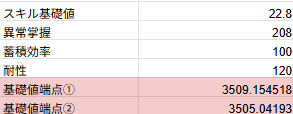
\includegraphics[width=0.7\linewidth]{ロームル1.png}
\end{frame}

%%%%%%%%%%%%%%%%%%%%%%%%%%%%%%%%%%%%%%%%%%%%%%%%%%%%%%%%%%%%%%%%%%%%%%%%
\begin{frame}{敵の異常蓄積値上限の近似方法}
そこでダメージボーナスや異常マスタリーなどもバフをして情報量を増やしてみる.
バフによる増加量をそれぞれ $\Delta x, \Delta y, \Delta z$とすると, 攻撃力, ダメージボーナス, 異常マスタリーの加重平均 $\bar{X}, \bar{Y}, \bar{Z}$ は
\[
\begin{aligned}
\bar{X}
&=
\frac{
  tX + (T-t)(X+\Delta x)
}{
  T
}
=
X + \left(1-\frac{t}{T}\right)\Delta x,
\\[0.8em]
\bar{Y}
&=
\frac{
  tY + (T-t)(Y+\Delta y)
}{
  T
}
=
Y + \left(1-\frac{t}{T}\right)\Delta y,
\\[0.8em]
\bar{Z}
&=
\frac{
  tZ + (T-t)(Z+\Delta z)
}{
  T
}
=
Z + \left(1-\frac{t}{T}\right)\Delta z
\end{aligned}
\]
となる.
\end{frame}
%%%%%%%%%%%%%%%%%%%%%%%%%%%%%%%%%%%%%%%%%%%%%%%%%%%%%%%%%%%%%%%%%%%%%%%%
\begin{frame}{敵の異常蓄積値上限の近似方法}
計算ダメージは

\[
\begin{aligned}
d
&=
C
\bar{X}
\frac{\bar{Y}}{100}
\frac{\bar{Z}}{100}
\\
&=
\frac{C}{10000}
\left\{
X+\left(1-\frac{t}{T}\right)\Delta x
\right\}
\left\{
Y+\left(1-\frac{t}{T}\right)\Delta y
\right\}
\left\{
Z+\left(1-\frac{t}{T}\right)\Delta z
\right\}
\end{aligned}
\]

となる.
ここで,

\[
C'=\frac{C}{10000},
\qquad
w=\frac{t}{T}
\]

とおくと,

\[
d
=
C'
\{X+(1-w)\Delta x\}
\{Y+(1-w)\Delta y\}
\{Z+(1-w)\Delta z\}
\]

となる.

\end{frame}

%%%%%%%%%%%%%%%%%%%%%%%%%%%%%%%%%%%%%%%%%%%%%%%%%%%%%%%%%%%%%%%%%%%%%%%%
\begin{frame}{敵の異常蓄積値上限の近似方法}
計算ダメージ $d$ を相対値 $w$ の関数 $d=d(w)$ とみなす.
定義域は $0 \le w \le 1$ とする.
計算ダメージと表示ダメージ端点との差を表す関数
\[
\begin{aligned}
F(w) &=d(w)-D \\
G(w)&=d(w)-(D-1)
\end{aligned}
\]
が $0 \le w \le 1$ 上で $0$ になる $w$ の近似値を2分法で求める.
以下を仮定すると $F, G$ はともに $0 \le w \le 1$上で単調減少であることから, $0 \le w \le 1$ 上でただ1つの解をもつことが分かる.
\begin{block}{仮定：表示ダメージの範囲}
表示ダメージはバフ前の計算ダメージより十分大きく, バフ後の計算ダメージより十分小さいとする. 
すなわち $d(1) \ll D-1<D \ll d(0)$ が成り立つとする. 
\end{block}

\end{frame}

%%%%%%%%%%%%%%%%%%%%%%%%%%%%%%%%%%%%%%%%%%%%%%%%%%%%%%%%%%%%%%%%%%%%%%%%
\begin{frame}{敵の異常蓄積値上限の近似方法}
\begin{block}{2分法による区間更新}
\small
初期区間を
\[
w_{\mathrm{L}}^{(0)}=0,
\qquad
w_{\mathrm{R}}^{(0)}=1
\]
とする.
第 $k$ 回目の中央点を
\[
w_{\mathrm{M}}^{(k)}
=
\frac{
w_{\mathrm{L}}^{(k)}+w_{\mathrm{R}}^{(k)}
}{2}
\]
とおき, $k+1$ 回目の端点を以下の場合分けで定める.
\[
\begin{array}{ll}
F(w_{\mathrm{L}}^{(k)})F(w_{\mathrm{M}}^{(k)})\le 0
&
\text{の場合}
\begin{cases}
w_{\mathrm{L}}^{(k+1)} = w_{\mathrm{L}}^{(k)}\\
w_{\mathrm{R}}^{(k+1)} = w_{\mathrm{M}}^{(k)}
\end{cases}
\\[1.2em]
F(w_{\mathrm{L}}^{(k)})F(w_{\mathrm{M}}^{(k)})>0
&
\text{の場合}
\begin{cases}
w_{\mathrm{L}}^{(k+1)} = w_{\mathrm{M}}^{(k)}\\
w_{\mathrm{R}}^{(k+1)} = w_{\mathrm{R}}^{(k)}
\end{cases}
\end{array}
\]
\end{block}

\end{frame}

%%%%%%%%%%%%%%%%%%%%%%%%%%%%%%%%%%%%%%%%%%%%%%%%%%%%%%%%%%%%%%%%%%%%%%%%
\begin{frame}{敵の異常蓄積値上限の近似方法}
\small
2分法を $n$ 回行った後の区間幅は,

\[
w_{\mathrm{R}}^{(n)}-w_{\mathrm{L}}^{(n)}
=
\frac{
w_{\mathrm{R}}^{(0)}-w_{\mathrm{L}}^{(0)}
}{
2^n
}
=
\frac{1}{2^n}
\]

となる.
そこで近似解を

\[
w
=
\frac{
w_{\mathrm{L}}^{(n)}+w_{\mathrm{R}}^{(n)}
}{
2
}
\]

とすると, この近似誤差は最大でも

\[
\left|
w-
\frac{
w_{\mathrm{L}}^{(n)}+w_{\mathrm{R}}^{(n)}
}{
2
}
\right|
\le
\frac{
w_{\mathrm{R}}^{(n)}-w_{\mathrm{L}}^{(n)}
}{
2
}
=
\frac{1}{2^{n+1}}
\]
である.

\end{frame}
%%%%%%%%%%%%%%%%%%%%%%%%%%%%%%%%%%%%%%%%%%%%%%%%%%%%%%%%%%%%%%%%%%%%%%%%
\begin{frame}{敵の異常蓄積値上限の近似方法}

十分大きい $n$ に対してこのように求めた $F(w)=0,G(w)=0$ の近似解をそれぞれ $w_{F}, w_{G}$ とすると, \[
d(w_{G}) < d(w) \le d(w_{F})
\]
が期待される(数学的な厳密解では成り立つ一方, 近似解ではもう少し精査が必要だが, 簡単のためここでは近似解でも成り立つと仮定する).

計算ダメージ $d$ は  $0 \le w \le 1$ 上単調減少なので, 相対値$w$の範囲は 
\[
w_{F}\le w < w_{G}
\]
となる. 
従って敵の異常蓄積値 $T$ の範囲は以下の通り
\[
\frac{t}{w_{G}}< T \le \frac{t}{w_{F}}.
\]

\end{frame}

\begin{frame}{敵の異常蓄積値上限の近似方法}

繰り返し回数 $n$ を $70$, アリアの「【ダッシュ攻撃】レガートステップ」の基礎値 $t=20.81$, 表示ダメージ $D=4048310$ と次のスライドにまとめた因子を用いて求めた「血狩りの掃除屋」の異常蓄積値上限の範囲は以下の通り.
\[
3506.237931...
<
T
\le
3506.279388...
\]

まだ精度が高いとは言えないが, この程度の誤差ならダメージ計算には大きな影響は与えない.
ここでは雑に平均をとって $3506.25$ とする.
また, 侵蝕 $1$ 回ごとに $2\%$ ずつ増加していくとする.
\end{frame}

\begin{frame}{敵の異常蓄積値上限の近似方法}
\begin{block}{使用した値}
\small
\begin{tabularx}{\linewidth}{@{}l l X@{}}
項目 & 値 & 式での扱い \\
\midrule
攻撃力 & $2903 \rightarrow 6028.75$ 
& $X=2903,\quad \Delta x=3125.75$ \\
\midrule
ダメージボーナス & $130 \rightarrow 249$
& $Y=130,\quad \Delta y=119$ \\
\midrule
異常マスタリー & $544 \rightarrow 649$
& $Z=544,\quad \Delta z=105$ \\
\midrule
防御補正 & $0.6339828$
& $C'$ に含める \\
\midrule
ダメージ倍率$\times$ レベル補正 & $125$
& $C'$ に含める \\
\midrule
狂咲倍率 & $1461.075$
& $C'$ に含める \\
\midrule
属性耐性 & $120$
& $C'$ に含める \\
\midrule
ブレイク倍率 & $180$
& $C'$ に含める \\
\midrule
別枠乗算 & $172.5$
& $C'$ に含める \\
\bottomrule
\end{tabularx}
\end{block}
\end{frame}
\end{document}
